% COMMENT THIS OUT TO HIDE SOLUTIONS
\def\SHOWSOLUTIONS{}

\documentclass[12pt]{article}

\usepackage[hidelinks]{hyperref}
\usepackage{comment}
\usepackage{color,graphicx,amsthm,amssymb,amsmath,cite,xspace,setspace}
\usepackage[small,bf]{caption}
\usepackage{multicol,multirow}
\usepackage{algorithm,algorithmic}
\usepackage{soul}
\usepackage{colortbl}
\usepackage{rotating}
\usepackage{textcomp}
\usepackage{epsf}
\usepackage{wasysym}
\usepackage{mdwtab}
\usepackage{bm}
\usepackage{verbatimbox}
\usepackage{framed} % To be able to frame theorems and stuff
\usepackage{subcaption}

\usepackage{tikz}
\usepackage{pgfplots}
\pgfplotsset{compat=1.17}


\usepackage{listings}
\definecolor{dkgreen}{rgb}{0,0.6,0}
\definecolor{gray}{rgb}{0.5,0.5,0.5}
\definecolor{mauve}{rgb}{0.58,0,0.82}

\lstset{frame=single,
	aboveskip=3mm,
	belowskip=3mm,
	basicstyle={\ttfamily},
	keywordstyle=\color{blue},
	commentstyle=\color{dkgreen},
	stringstyle=\color{mauve},
	tabsize=3
}


% solutions
\newenvironment{solution}{\vspace{2mm}\color{blue}\textbf{Solution: }}{\color{black}}
\ifdefined\SHOWSOLUTIONS\else\excludecomment{solution}\fi

% define the type of list to use
\usepackage[shortlabels]{enumitem}
\setlist[enumerate,1]{\bfseries 1., itemsep=6mm}
\setlist[enumerate,2]{\bfseries a), itemsep=3mm}

\def\wl{\par \vspace{\baselineskip}} 
\def \bx{\boldsymbol{x}}
\def \bw{\boldsymbol{w}}
\def \bnu{\boldsymbol{\nu}}
\def \by{\boldsymbol{y}}
\def \bz{\boldsymbol{z}}
\def \bu{\boldsymbol{u}}
\def \bv{\boldsymbol{v}}
\def \bb{\boldsymbol{b}}
\def \bg{\boldsymbol{g}}
\def \ba{\boldsymbol{a}}
\def \be{\boldsymbol{e}}
\def \bA{\boldsymbol{A}}
\def\bU{\boldsymbol{U}}
\def \bB{\boldsymbol{B}}
\def \bC{\boldsymbol{C}}
\def \bX{\boldsymbol{X}}
\def \bT{\boldsymbol{T}}
\def \bP{\boldsymbol{P}}
\def \bV{\boldsymbol{V}}
\def \bE{\boldsymbol{E}}
\def \bS{\boldsymbol{S}}
\def \bSigma{\boldsymbol{\Sigma}}
\def \bI{\boldsymbol{I}}

\def\R{{\mathbb R}}
\def\E{{\mathbb E}}
\def\P{{\mathbb P}}
\def \X{{\cal X}}
\def \Y{{\cal Y}}

\DeclareMathOperator{\rank}{rank}
\DeclareMathOperator{\Sign}{sign}
 

\usepackage{fullpage}

% Header and footer
\usepackage{fancyhdr,lastpage}
\pagestyle{fancy}
\cfoot{\thepage\ of \pageref{LastPage}}
\renewcommand{\headrulewidth}{0.0pt}
\renewcommand{\footrulewidth}{0.0pt}

\begin{document}
\begin{center}
{\large ECE 330: Signals \& Systems  -  Problem Set}
\mbox{ }\\
\mbox{ }\\
\end{center}



%\noindent \emph{Note: Please include the names of all the classmates with whom you have collaborated on this activity in your submission.} 

\begin{enumerate}[\qquad 1)]
    %Problem 1
    \index{Signals, MATLAB, Sketching}

    \item Sketch the following signals (check your work using MATLAB):
    \\ a) $u(t-5) - u(t-7)$
    \\ b) $u(t-5) + u(t-7)$
    \\ c) $t^2[u(t-1) - u(t-2)]$
    \\ d) $(t-4)[u(t-2) - u(t-4)]$
    \\ e) $2t(u(t+2) - u(t-1))$ 
    \\ f) \textbf{Bonus: } $\sum_{k=1}^{+\infty} (-1)^k (u(t - (k-1)) - u(t - k))$

    \begin{solution}
        \begin{figure}[htbp]
            \centering
            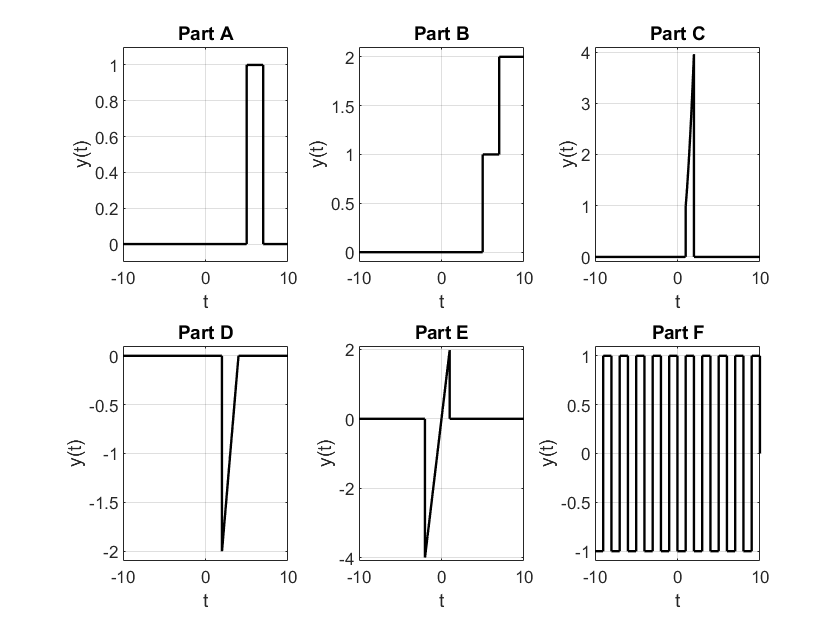
\includegraphics[width=0.8\textwidth]{images/problem2.png}
            \label{fig:Problem1}
        \end{figure}
    \end{solution}


    \newpage

    %Problem 2
    \index{Signals, Unit Step}

    \item Give an expression for the signal, $y(t)$, shown in the figure using the unit step function.

    \begin{figure}[htbp]
        \centering
        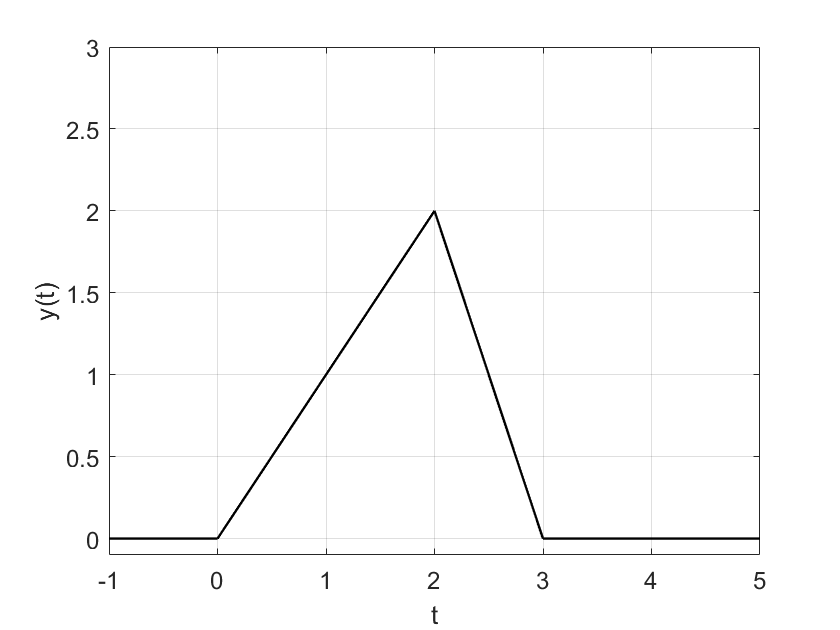
\includegraphics[width=0.8\textwidth]{images/problem3.png}
        \label{fig:Problem2}
    \end{figure}


    \begin{solution}
         The signal may be broken down into the sum of two separate signals: one for the rising portion and one for the decreasing portion. Both ramps are linear meaning the amplitude of the signal is proportional to $t$. Rising Ramp: $x_1(t) = t[u(t) - u(t-2)]$. Also, $u(t) - u(t-2)$ constrains the ramp from $0\leq t \leq 2$. Then, for the decreasing ramp, it is again linear but now proportional by $-2t$ and occurs in the interval $2 \leq t \leq 3$. Thus, the decreasing ramp: $x_2(t) = -2(t-3)[u(t-2) - u(t-3)]$. Finally: \[y_t(t) = y_1(t) + y_2(t) = tu(t) - 3(t-2)u(t-2) + 2(t-3)u(t-3)\]
    \end{solution}

    \newpage

    % Problem 3
    \index{Signals, MATLAB, Sketching}

    \item Give an expression for the following signal shown in the figure using the step function.
    
    \begin{figure}[htbp]
        \centering
        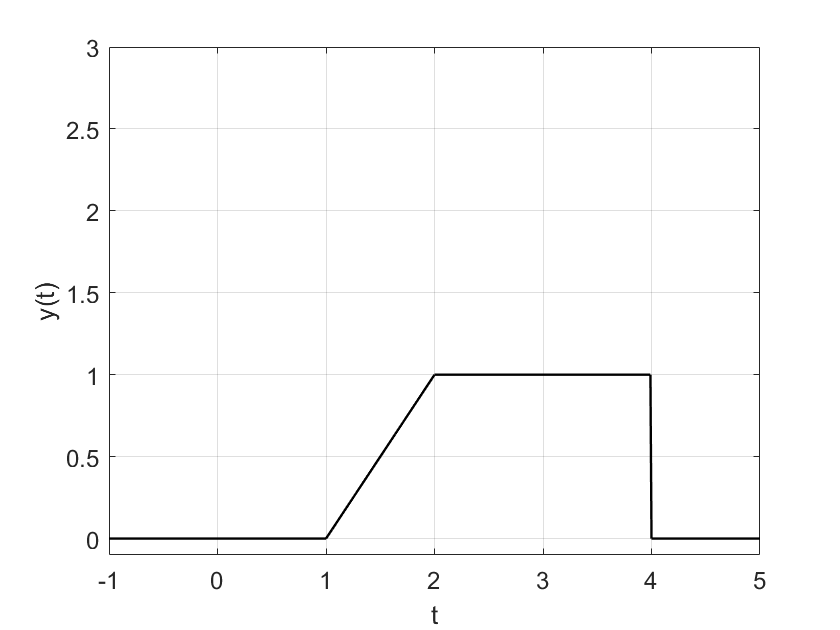
\includegraphics[width=0.8\textwidth]{images/problem4.png}
        \label{fig:Problem3}
    \end{figure} 

    \begin{solution}
         \[y(t) = (t-1)u(t-1) - (t-2)u(t-2)-u(t-4)\]
        Each term in the solution serves a specific role in the visual characteristic of the signal. The first term, $(t-1)u(t-1)$ acts as the increasing ramp in the interval $1 \leq t \leq 2$. \par
        Then, the following term $(t-2)u(t-2)$ cancels out the increasing ramp for $t > 2$. Lastly, $u(t-4)$ gives us the familiar rectangle ending at $t=4$.
    \end{solution}

    \newpage

    % Problem 4
    \index{Signals, Unit Step}

    \item Simplify the following expressions containing the unit step:
    
    a) $(t^3 + 3)\delta(t)$

    b) $[sin(t^2 - \frac{\pi}{2})\delta(t)]$

    c) $e^{-2t}\delta(t)$

    d) $\frac{\omega^2 + 1}{\omega^2 + 9}\delta(\omega - 1)$

    \begin{solution}
        \\
        a) $3\delta(t)$

        b) $-\delta(t)$

        c) $\delta(t)$

        d) $\frac{1}{5}\delta(\omega - 1)$
    \end{solution}

    % Problem 5
    \index{Signals, Impulse}

    \item Simplify the following unit impulse expressions:
    
    a) $\int_{-\infty}^{\infty} \delta(t)e^{-j\omega t}dt $

    b) $\int_{-\infty}^{\infty} \delta(t-2)cos(\frac{\pi t}{4}) dt $

    c) $\int_{-\infty}^{\infty} e^{-2(x-t)}\delta(2-t)dt $

    \begin{solution}
        \\
        a) $1$

        b) $0$

        c) $e^{-2(x-2)}$
    \end{solution}

\newpage
\section*{Exercises}

\subsection*{Time Invariance}

Recall that time invariance refers to a system where if the input is delayed by T seconds, the output is the same as before but delayed by T. In other words, a signal is time invariant if a delay between the input and output does not affect the signals output.

\begin{figure}[htbp]
    \centering
    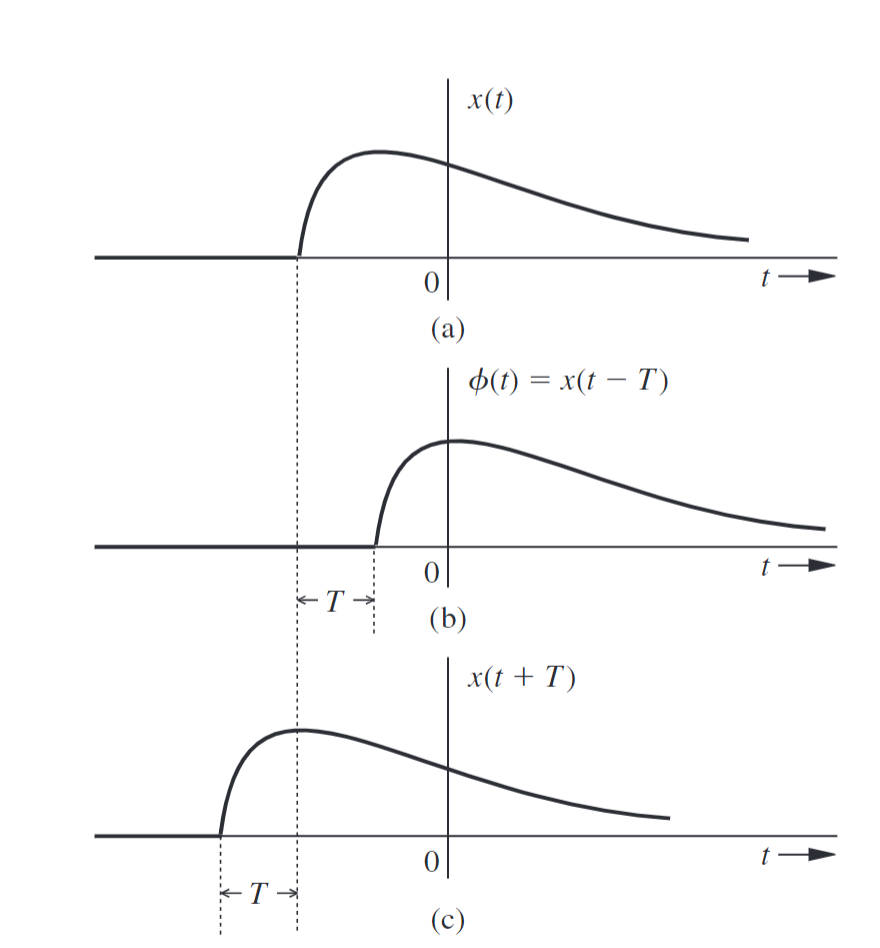
\includegraphics[width=0.4\textwidth]{images/TimeInvariance.png}
    \caption{Time Delay Example}
    \label{fig:Problem5}
\end{figure} 
    
Answer the following questions related time invariance of systems. Determine if the following systems are time invariant.  \textbf{Show your work}.

(Hint: If you suspect time variance, use an example to show the system fails to satisfy the time-invariance property).

a) $y(t) = x(t)u(t)$\\

b) $y(t) = \frac{d}{dt}x(t)$\\

c) $y(t) = sin(t)x(t-2)$

\begin{solution}
    \\
    a) This system is time variant. We can show this using a counter example. Let $x(t) = \delta(t + 1)$. We see that $y(t) = 0$. Now, by applying a delay to our input, we have $x(t-2) = \delta(t - 1)$ which means our new output is $y(t-2) = \delta(t-1)$ which does not equal our output without the delay. 
    \\
    b) This system is time invariant. Lets apply a delay to our input which gives us $y(t-T) = \frac{d}{d(t-T)}x(t-T) = \frac{d}{dt}x(t-T)$ which is just the output of the system to a delayed input.
    \\
    c) This system is time variant. If we apply a delay, we see that $y(t-T) = sin(t-T)x(t-2-T)$. If $sin(t)$ does not equal $sin(t-T)$ then the system is time variant. 
\end{solution}

\newpage
\subsection*{Sampling and Reconstruction}

Let the $T$-periodic wave $s(t)$ be defined as

\[s(t) = \begin{cases}
    1, & |t| < T_0 \\
    0, & T_0 < |t| < T/2 \\
    s(t+T), & \forall t
    \end{cases}\]

Now, define the product of $s(t)$ and some arbitrary waveform $x(t)$ as $v(t) = x(t)s(t)$. We can treat this product as a continuous time sampling of $x(t)$ where portions of $x(t)$ associated with the zero parts of $x(t)$ are eliminated. 

This is shown in the figure below.

\begin{figure}[htbp]
    \centering
    % Top row
    \begin{subfigure}[t]{0.48\textwidth}
        \centering
        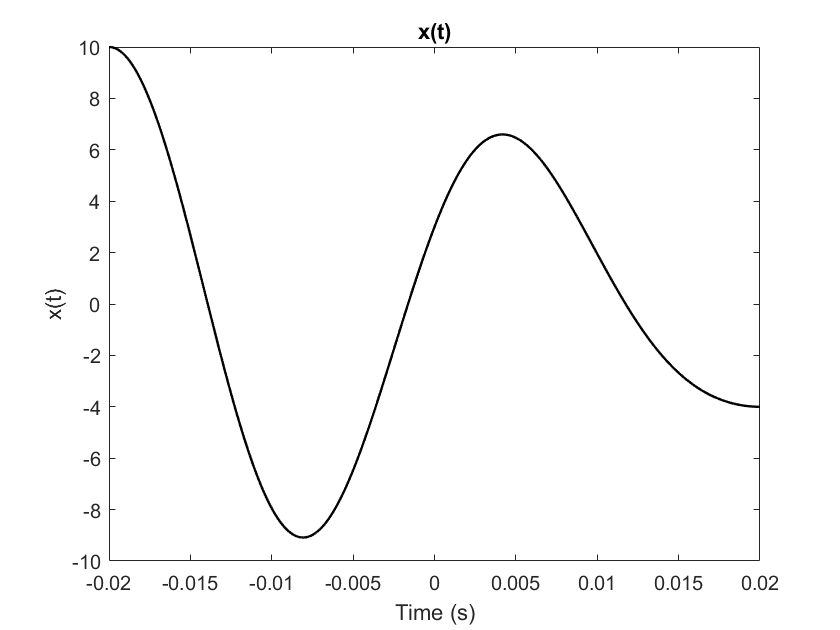
\includegraphics[width=1.0\textwidth]{images/xt.png}
        \caption{$x(t)$ is some arbitrary signal.}
        \label{fig:image1}
    \end{subfigure}
    \begin{subfigure}[t]{0.48\textwidth}
        \centering
        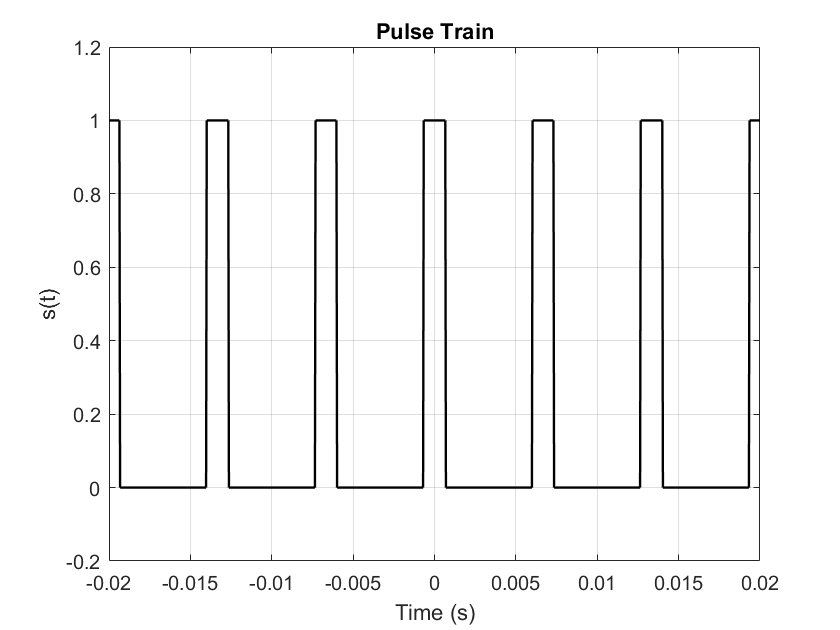
\includegraphics[width=1.0\textwidth]{images/pulseTrain.png}
        \caption{Pulse train representing our sampling.}
        \label{fig:image2}
    \end{subfigure}

    \vspace{0.5em}

    % Bottom row
    \begin{subfigure}[t]{0.48\textwidth}
        \centering
        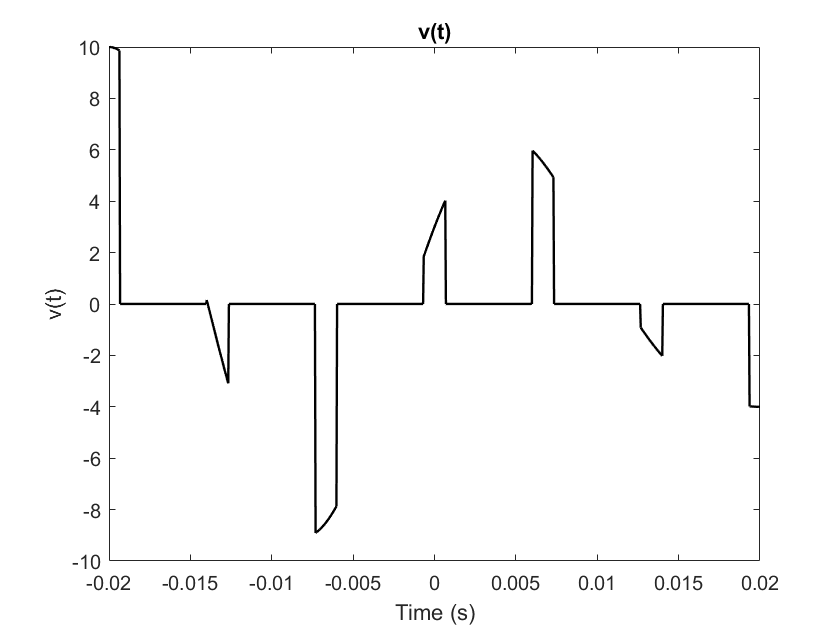
\includegraphics[width=1.0\textwidth]{images/vt.png}
        \caption{$v(t)$ representing our sampled signal.}
        \label{fig:image3}
    \end{subfigure}
    \begin{subfigure}[t]{0.48\textwidth}
        \centering
        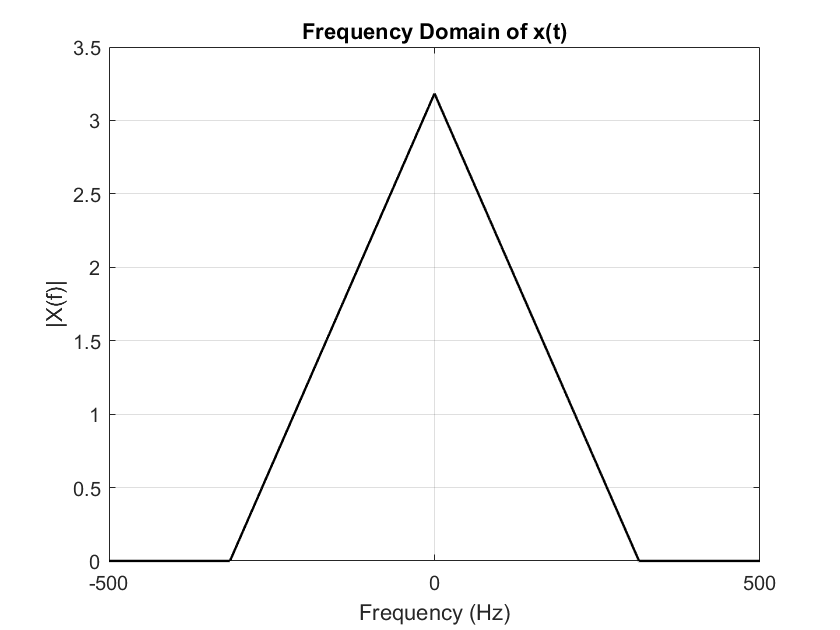
\includegraphics[width=1.0\textwidth]{images/reconstructionXofT.png}
        \caption{Frequency domain of $x(t)$. The nonzero portion ranges from $[-100\pi, 100\pi]$.}
        \label{fig:image4}
    \end{subfigure}

    \label{fig:reconstruction}
\end{figure}

We will assume the Fourier transform of $x(t)$ is a simple triangular spectrum as depicted in the figure above. Let the nonzero band be defined between $-W < \Omega < W$ where $W = 100\pi$ rads/sec.

Begin by finding $S(\Omega)$, the Fourier transform representation of $s(t)$.
Assume that $T = 1/150$ and $T_0 = 1/1500$.

\begin{solution}
    
\end{solution}

Use the multiplication in time-convolution in frequency property of the Fourier transform to find the expression for $V(\Omega)$. Sketch $V(\Omega)$ and answer the following questions.

What is the minimum $T$ for which the portions of $V(\Omega)$ do not overlap?

\begin{solution}
    $\frac{2\pi}{T} > 2W$
\end{solution}

Now pass $v(t)$ through a low pass filter with impulse response

\[h(t) = (\frac{T}{2T_0})\frac{sin(100\pi t)}{\pi t}\]

to obtain $y(t) = v(t) * h(t)$. what is the output of the filter? \textbf{Hint: use the convolution in time-multiplication in frequency property.}

\begin{solution}
    $y(t) = x(t)$
\end{solution}

\end{enumerate}
\end{document}
